Here we describe the process of building the FPGA timetagging
unit. This will require the materials listed in \ref{Ch:BoM}.  The
time-tagger is built around an the Xylo EM development board. This
board provides a Altera Cyclone Field-Programmable Gate Array (FPGA)
as well as a device (the Cypress FX2) for interfacing with a
traditional USB bus. The FPGA consists of a set of logic elements
(e.g. boolean logic gates), memories, and buses which can be connected
to form complex, high-speed digital devices.

Since the difficult work of supporting the FPGA logic is done for us
by the Xylo board, very little remains to be done. To keep out
electromagnetic interference, the board should be mounted in a metal
enclosure. While the size depends upon the number of desired channels,
we find that a 6x6x6 inch box provides ample space. Additionally, you
will need BNC connectors and cable to couple signals on to the board,
as well as stand-offs and bolts for mounting the board in the
box. Four channels is probably a good starting point.

\begin{figure}
  \center
  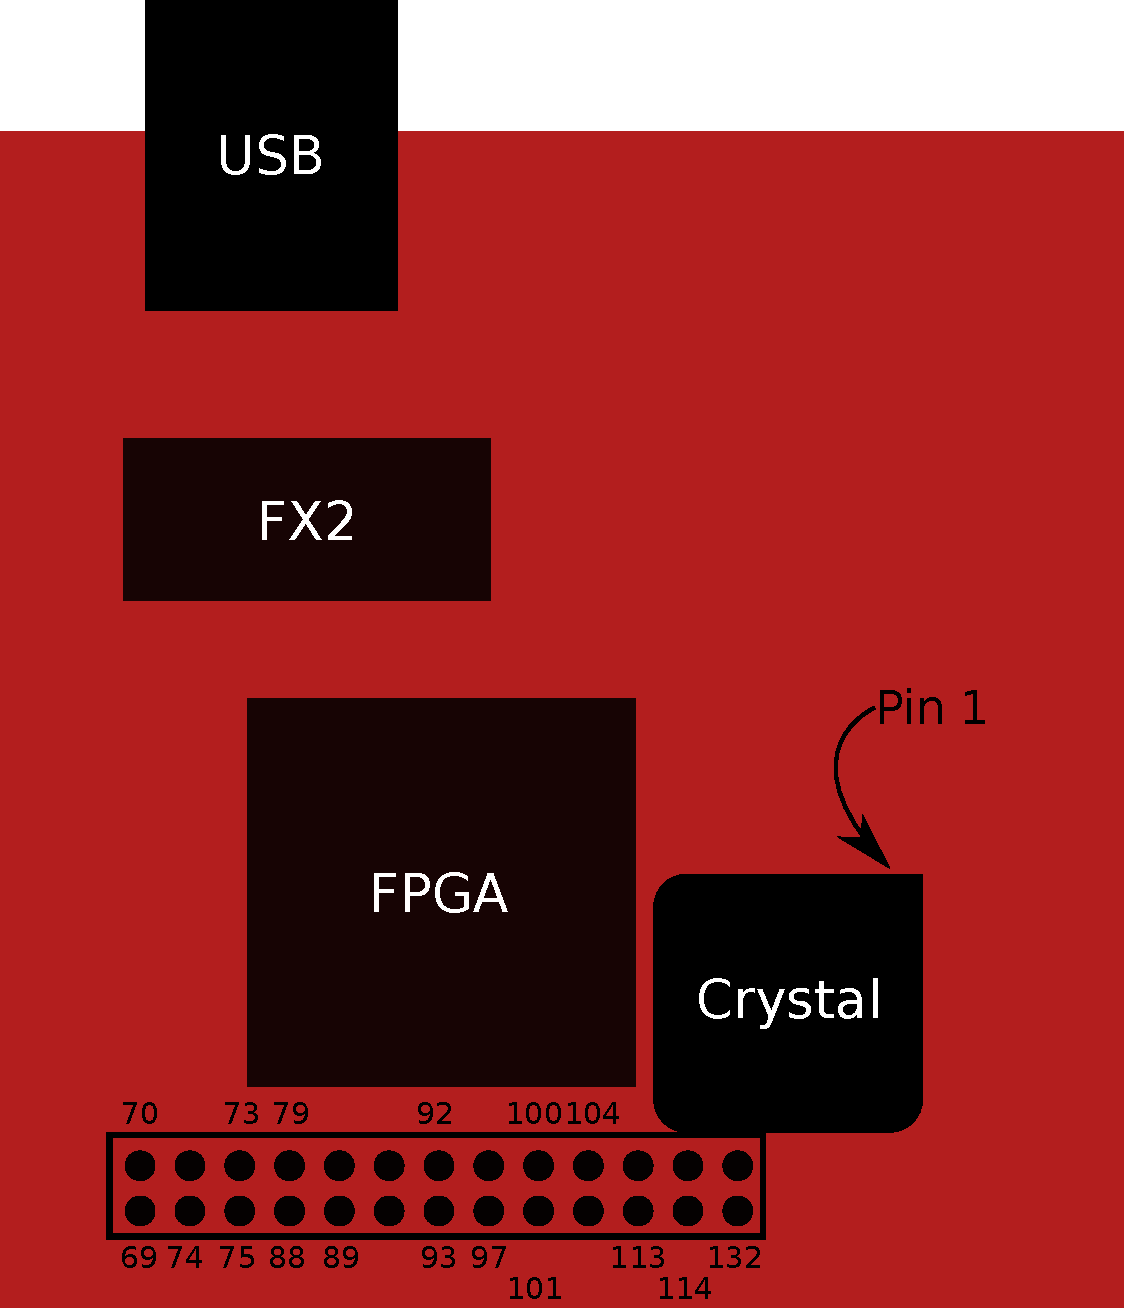
\includegraphics[scale=0.5]{board-schematic.pdf}
  \caption{A schematic depiction of the Xylo EM FPGA development board}
  \label{fig:board-schematic}
\end{figure}

\section{Preparing the box}

To mount the board and connectors in the box, several holes will need
to be drilled. At very least, you will need holes for,

\begin{itemize}
  \item The board's USB connector
  \item The board's four mounting screws 
  \item The BNC connectors
\end{itemize}

One possible connector arrangement is shown in Figure
\ref{fig:front-panel}.

\begin{figure}
  \center
  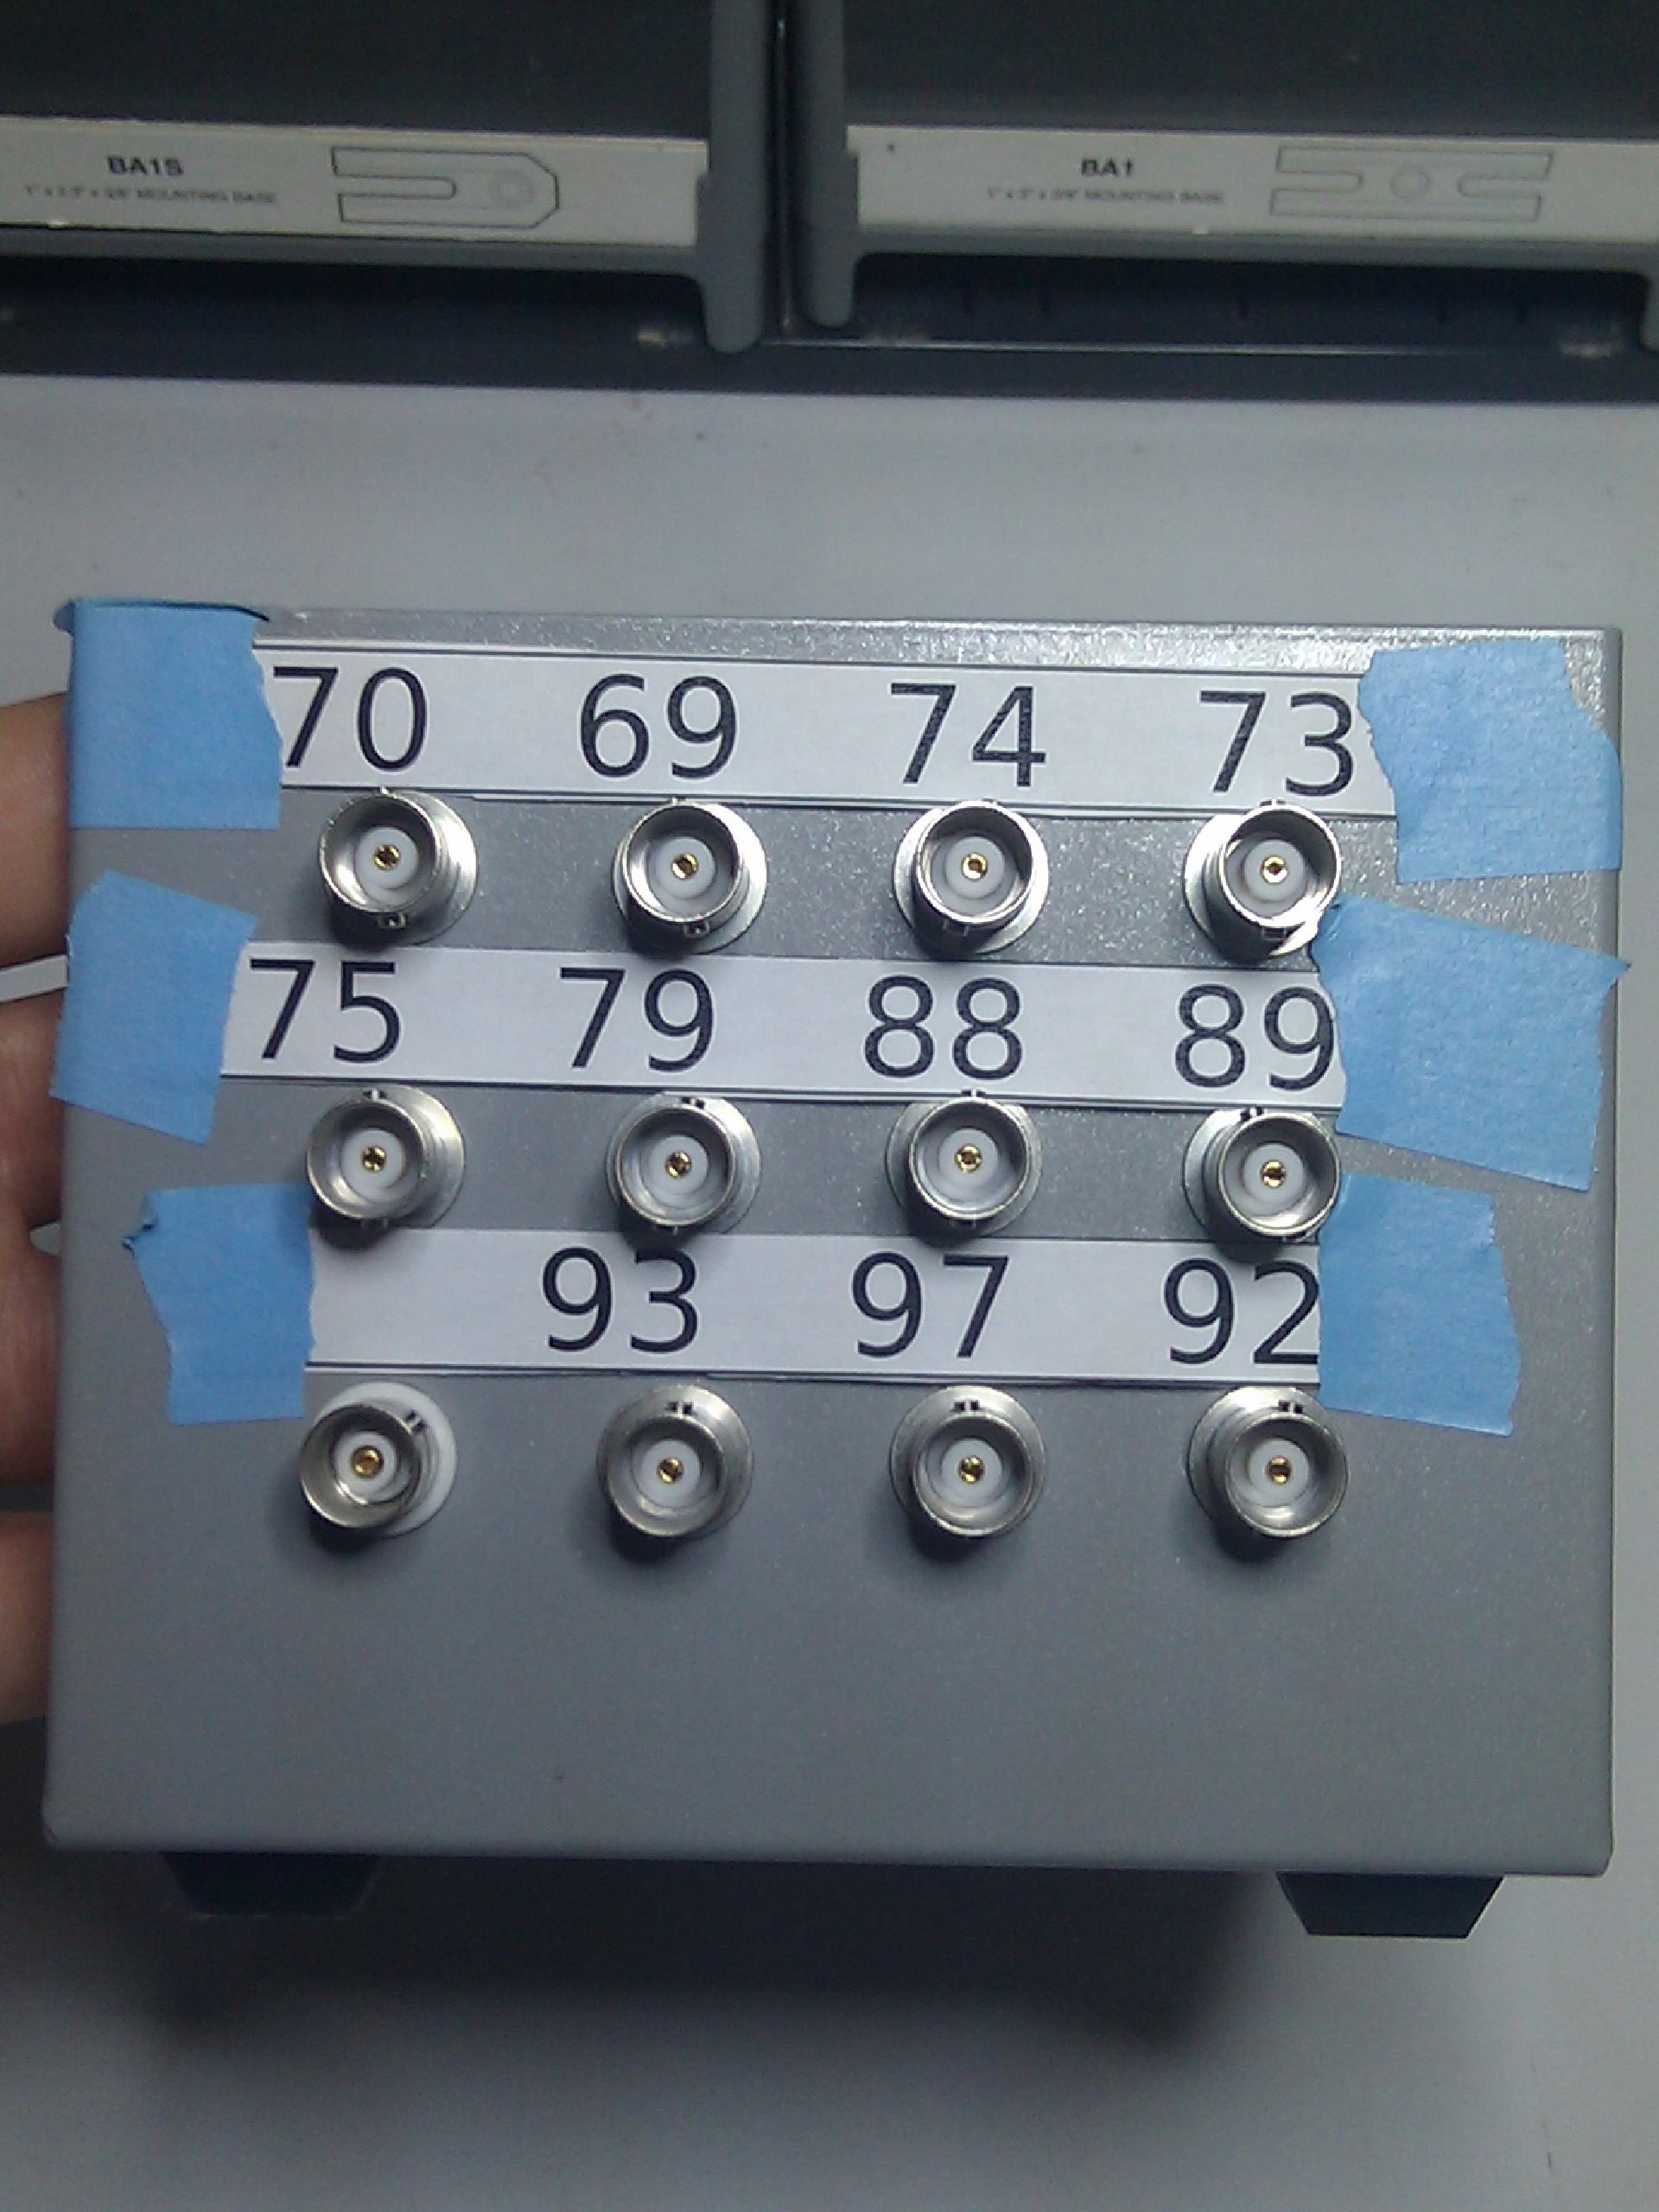
\includegraphics[scale=0.2]{front-panel.jpeg}
  \caption{One possible BNC connector arrangement}
  \label{fig:front-panel}
\end{figure}

\begin{figure}
  \center
  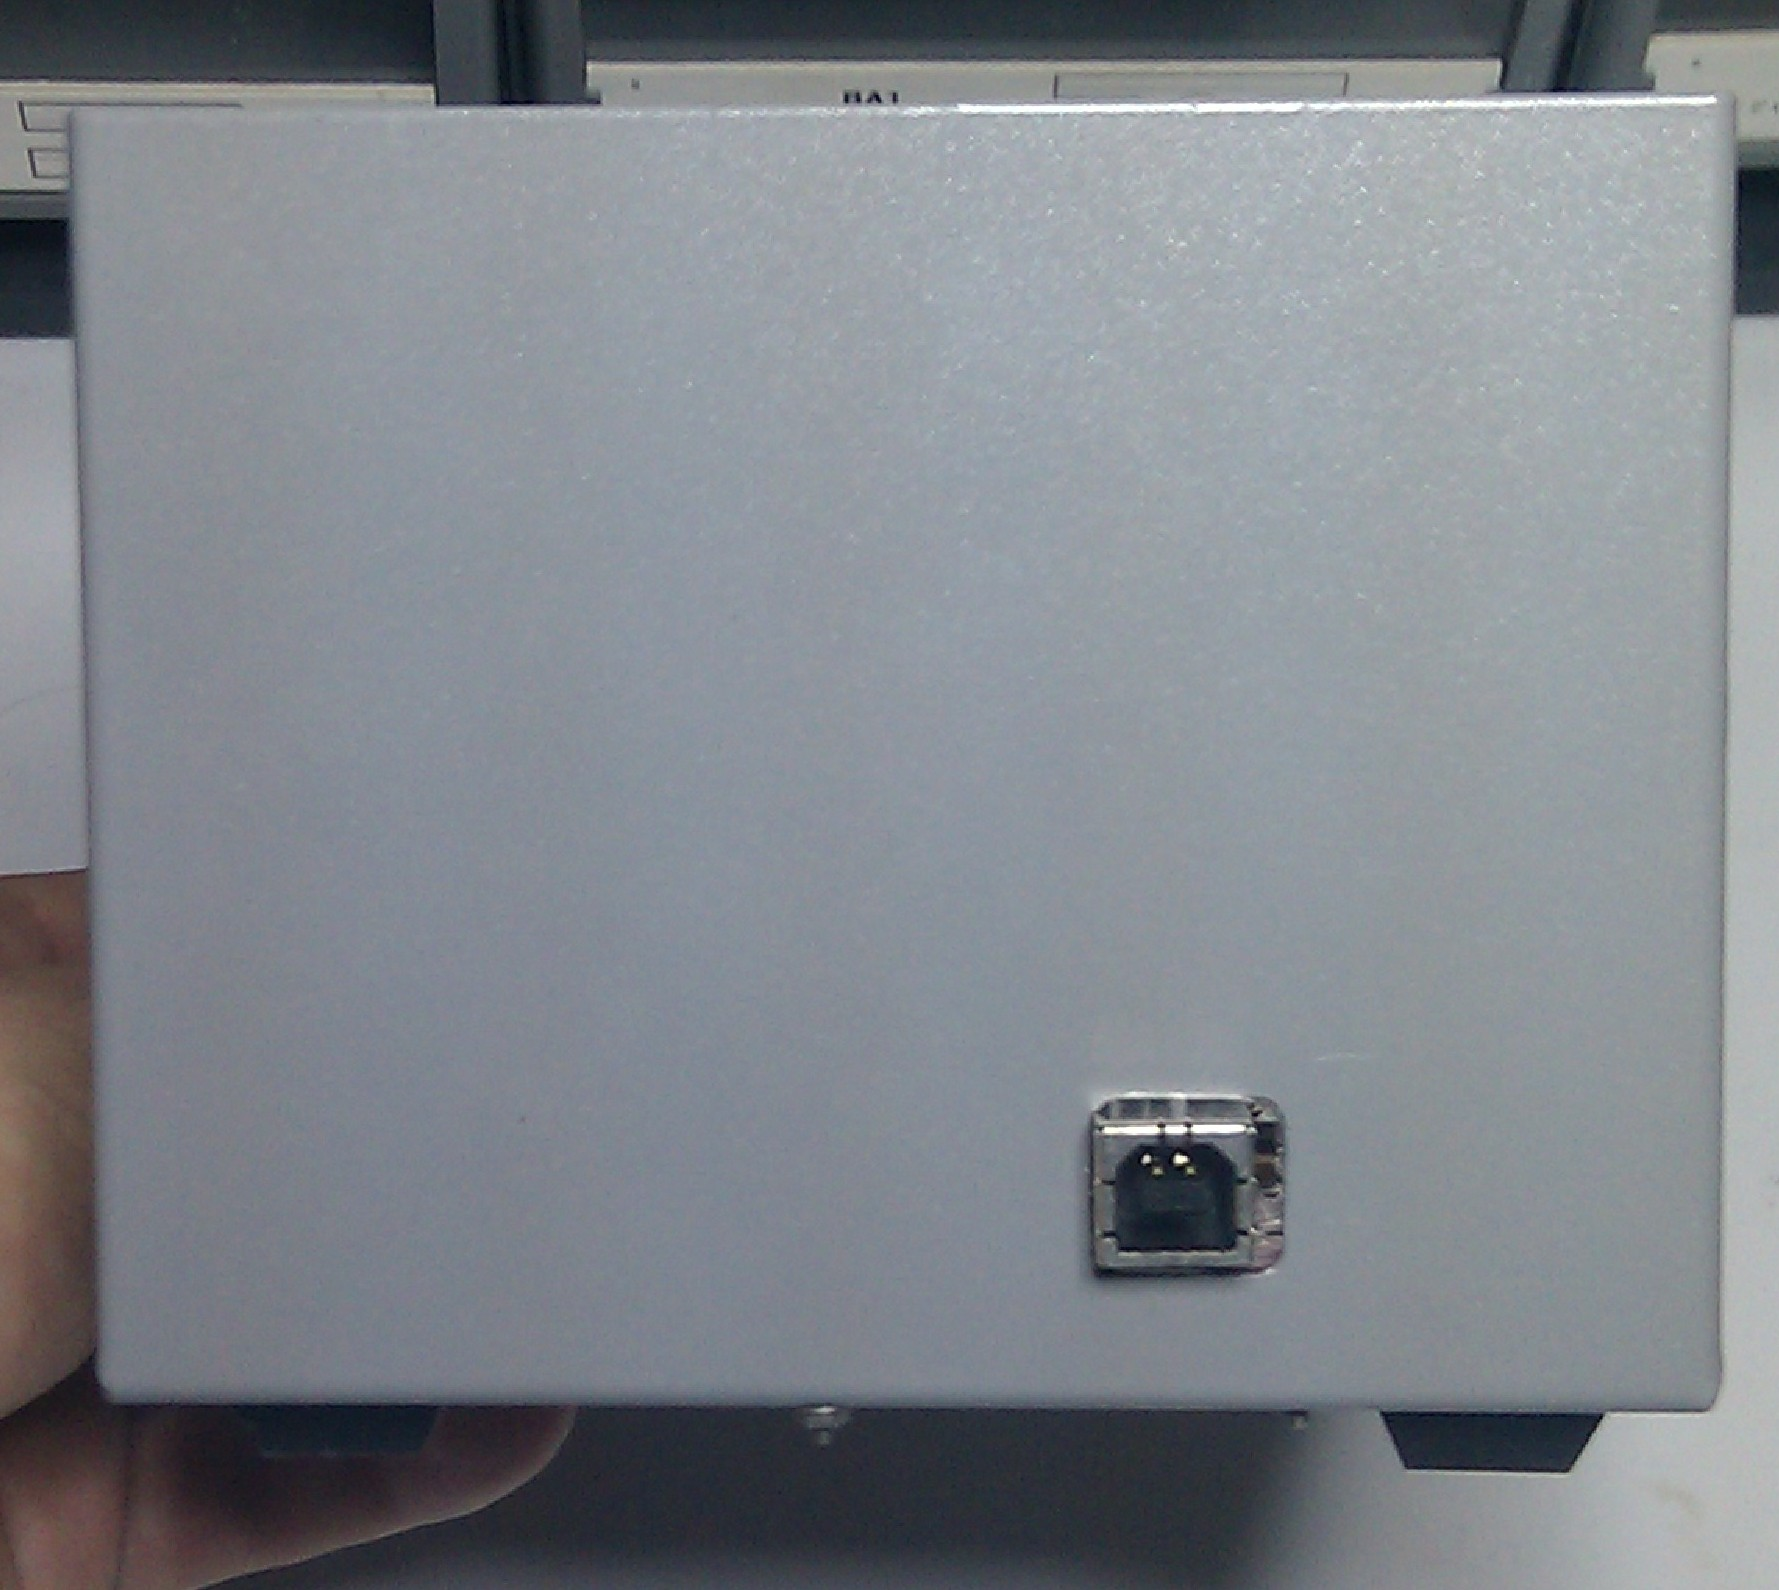
\includegraphics[scale=0.1]{box-rear.jpeg}
  \caption{Rear of the box with cut-out for USB connector}
  \label{fig:box-rear}
\end{figure}

\section{Connectors}

\subsection{Some notes on soldering}

While none of the soldering required in the construction of this board
is particularly difficult, it is important that proper soldering
technique is observed. At best, improperly made solder joints will be
mechanically and electrically unstable. At worst, damage to the board
could result. It is important to know the type of solder you are
working with and its characteristics before commencing.

In particular, you want either a 60-40 tin-lead or ROHS-compliant
lead-free solder with rosin. It is critical that the 
solder used is intended for electrical applications and not plumbing.

Before a joint is made, it is crucial that both surfaces are
clean. Gently scrubbing with a cotton swab soaked in methanol should
remove most organic matter. Moreover, the metal surfaces of most
electronic parts will quickly form an oxide layer on exposure to
air. This layer will make soldering extremely difficult unless removed
by a flux. While the rosin in a rosin-core solder will help accomplish
this, more flux will only make things easier.

While a cheap unregulated iron can be used for making the less
sensitive joints of the instrument (e.g. cables), these units are
notoriously bad at maintaining a stable temperature and can easily
cause damage if misused while soldering on the sensitive Xylo
board. Instead, it is recommended that a regulated solder station is
used.

The station should be set at a temperature near the eutectic point of
the solder (typically around 250 degrees celcius). When making a
joint it is important not to be overly cautious about applying heat
and be certain that both surfaces are being heated: a joint cannot be
made without both surfaces being above the eutectic temperature.

Before making a joint, ensure that both surfaces being joined are
securely held in place.  To make a joint, begin by taking the iron,
clean the tip to remove residue and excess solder. Next, apply just
enough solder to cover the tip with a thin layer. This layer will
provide a medium to improve thermal contact between the tip and
surfaces being jointed. Next, bring the tip into contact with both
surfaces. After a second or so of contact, the surfaces should be
approaching the eutectic point of the solder, allowing the thin layer
applied earlier to wet. At least point, begin feeding solder wire to
the joint. It is important to provide enough solder to make a secure
joint while avoiding applying so much solder to make the join convex.

When a sufficient amount of solder has been applied, remove the iron
and allow the joint to cool. It is very important that the joint is
allowed to cool without being disturbed. Cooling with forced air,
moving the joined pieces or otherwise disturbing the joint at this
point can result in a "cold joint." While a proper solder joint will
appear shiny and strongly wetted to both surfaces, a cold joint will
have a hazy appearance and will often be poorly wetted. While a cold
joint may hold for a some time, it is far more likely that such a
joint will eventually fail, perhaps with only very subtle but no less
significant results.

Finally, after a joint is made, it is crucial that the flux residue
remaining on the board is removed. This usually must be dissolved with
an organic solvent (ethanol or methanol should work nicely). After
dissolving, the remaining residue can be removed by flushing with
water and gentle scrubbing (an old toothbrush works well). Failure to
remove flux residue can result in short circuits, unstable circuits,
and slow degradation of solder joints. Be sure to allow the board to
dry fully after removing the flux residue.

\subsection{Soldering the pin header}

In order to connect the BNC connectors to the board, a pin header
needs to be soldered to the board. The board has room for a $2 \times
13$ 0.1 inch spacing pin header directly beside the FPGA. This header
should be placed as shown in Figure \ref{fig:header} and soldered from
the back side of the board. Again, be sure to use care in soldering to
the board.

\begin{figure}
  \center
  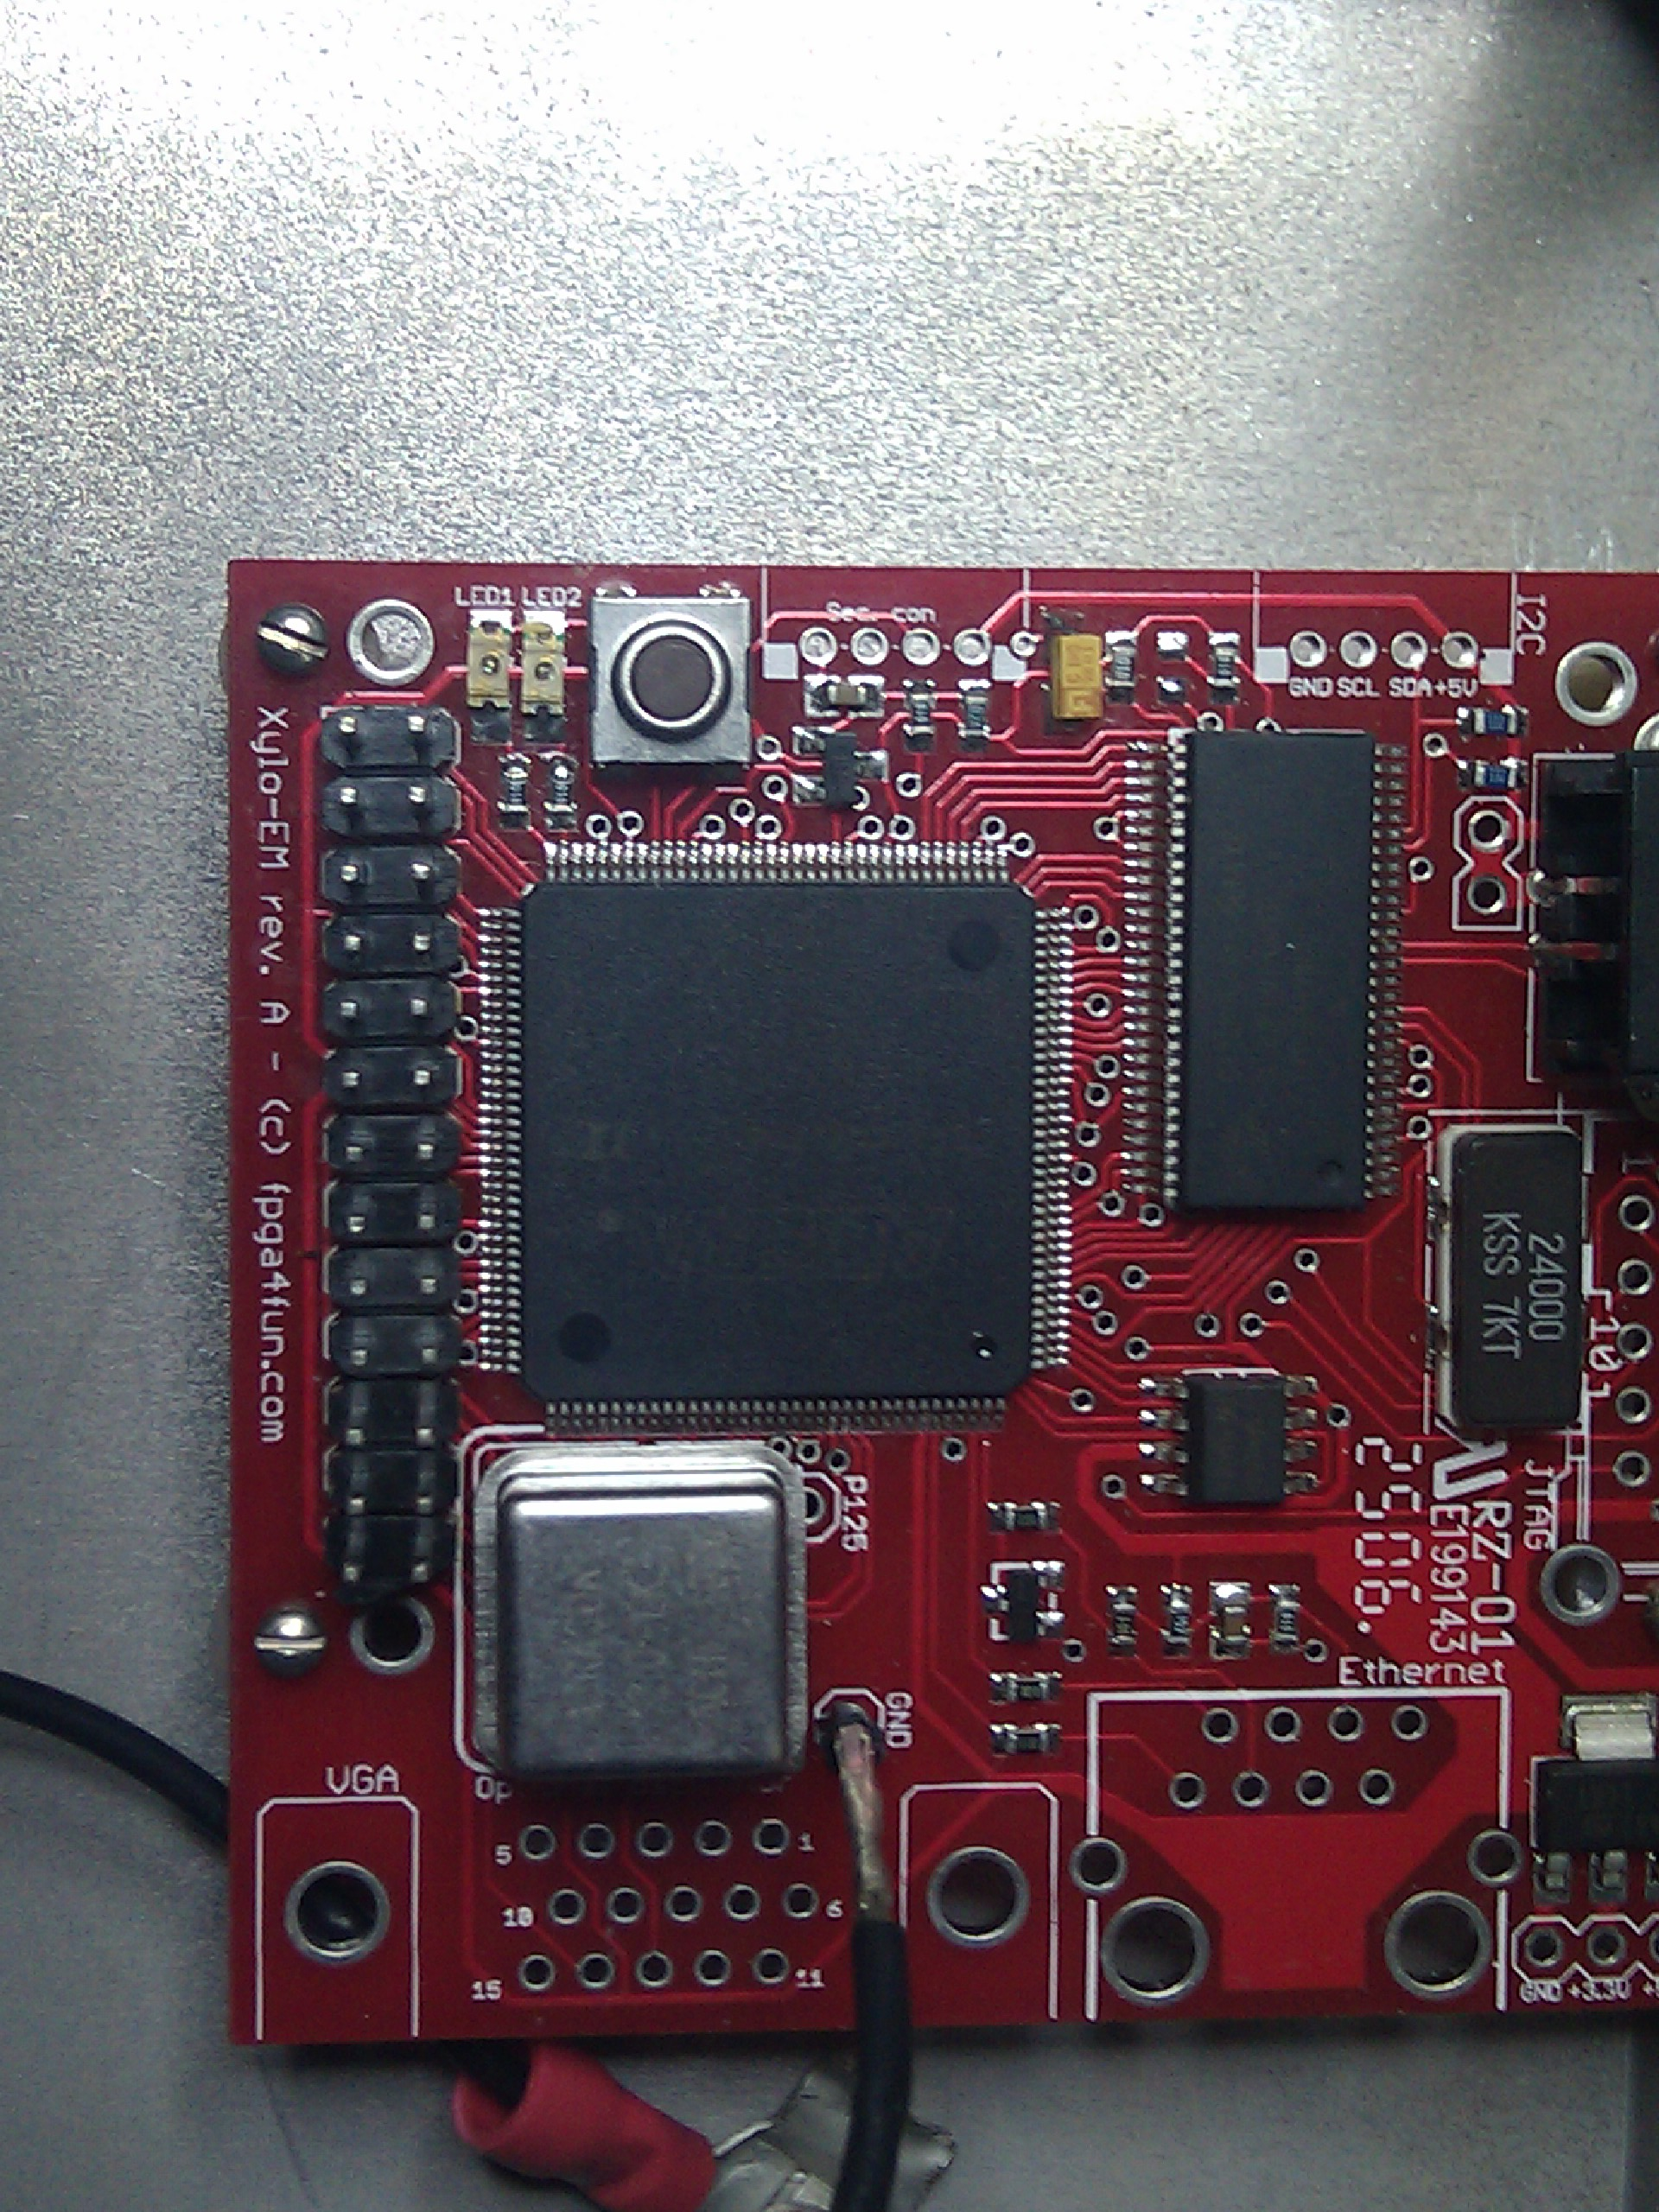
\includegraphics[scale=0.2]{board-header.jpeg}
  \caption{Placement of the pin headers}
  \label{fig:header}
\end{figure}

\section{BNC connectors}

Bulkhead BNC connectors are used to bring the signal from the outside
world to the FPGA board. You will need one connector for each desired
signal listed in Table \ref{table:pins}.

While unshielded single conductor wire can be used in a pinch, it is
recommended that coaxial cable is used to couple the BNC connectors to
the board.

It is important to note that there are two varieties of bulkhead BNC
connector: Isolated ground connectors and body-grounded. These can be
distinguished by the number of pins on the interior side of the
connector. Namely, body-grounded connectors will have a single
centrally located pin connected to the center conductor of the BNC
connector while an isolated ground connector will have an additional
ground pin. In the case of a body grounded connector, the signal
ground is shorted to the chassis in which the connector is mounted.

This distinction can have important consequences in the construction
of your instrument. To avoid ground loops, one must ensure there
exists exactly one path to ground from any given point in the circuit.
Three possible ground configurations are shown in Figure \ref{fig:grounding}.

\begin{figure}
  \center
  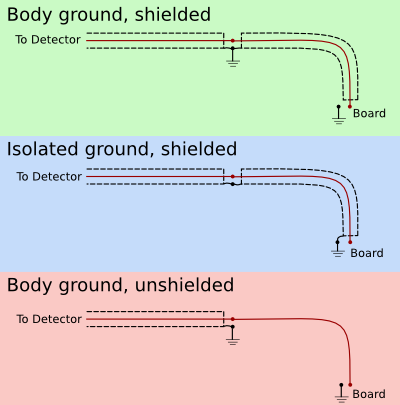
\includegraphics[scale=0.3]{bnc-grounding.png}
  \caption{Three possible grounding configurations}
  \label{fig:grounding}
\end{figure}

In the first configuration a isolated ground connector is used,
allowing the the signal ground to be coupled to the board ground
at the board. This gives rise to a star topology which is best
from the perspective of signal integrity since current from one signal
to ground are unable to affect the ground potential of another signal,
assuming the grounds meet at a low impedence junction.

The second configuration is recommended if body grounded connectors
are used. Here, all signal grounds are coupled through the metal
box. In addition, the shielding of the coaxial run from connector to
the board is also grounded to the box, providing shielding between
signals. The coax ground is left disconnected on the board side to
avoid creating a ground loop.

The third configuration is also acceptable, solving the multiple
ground problem by simply neglecting the grounded shielding from the
connector to the board.

Once a grounding configuration has been decided upon, installation of
the connectors is quite simple. One possible configuration (employing
grounding scheme 3) is shown in Figure \ref{fig:front-panel-rear}.

\begin{figure}
  \center
  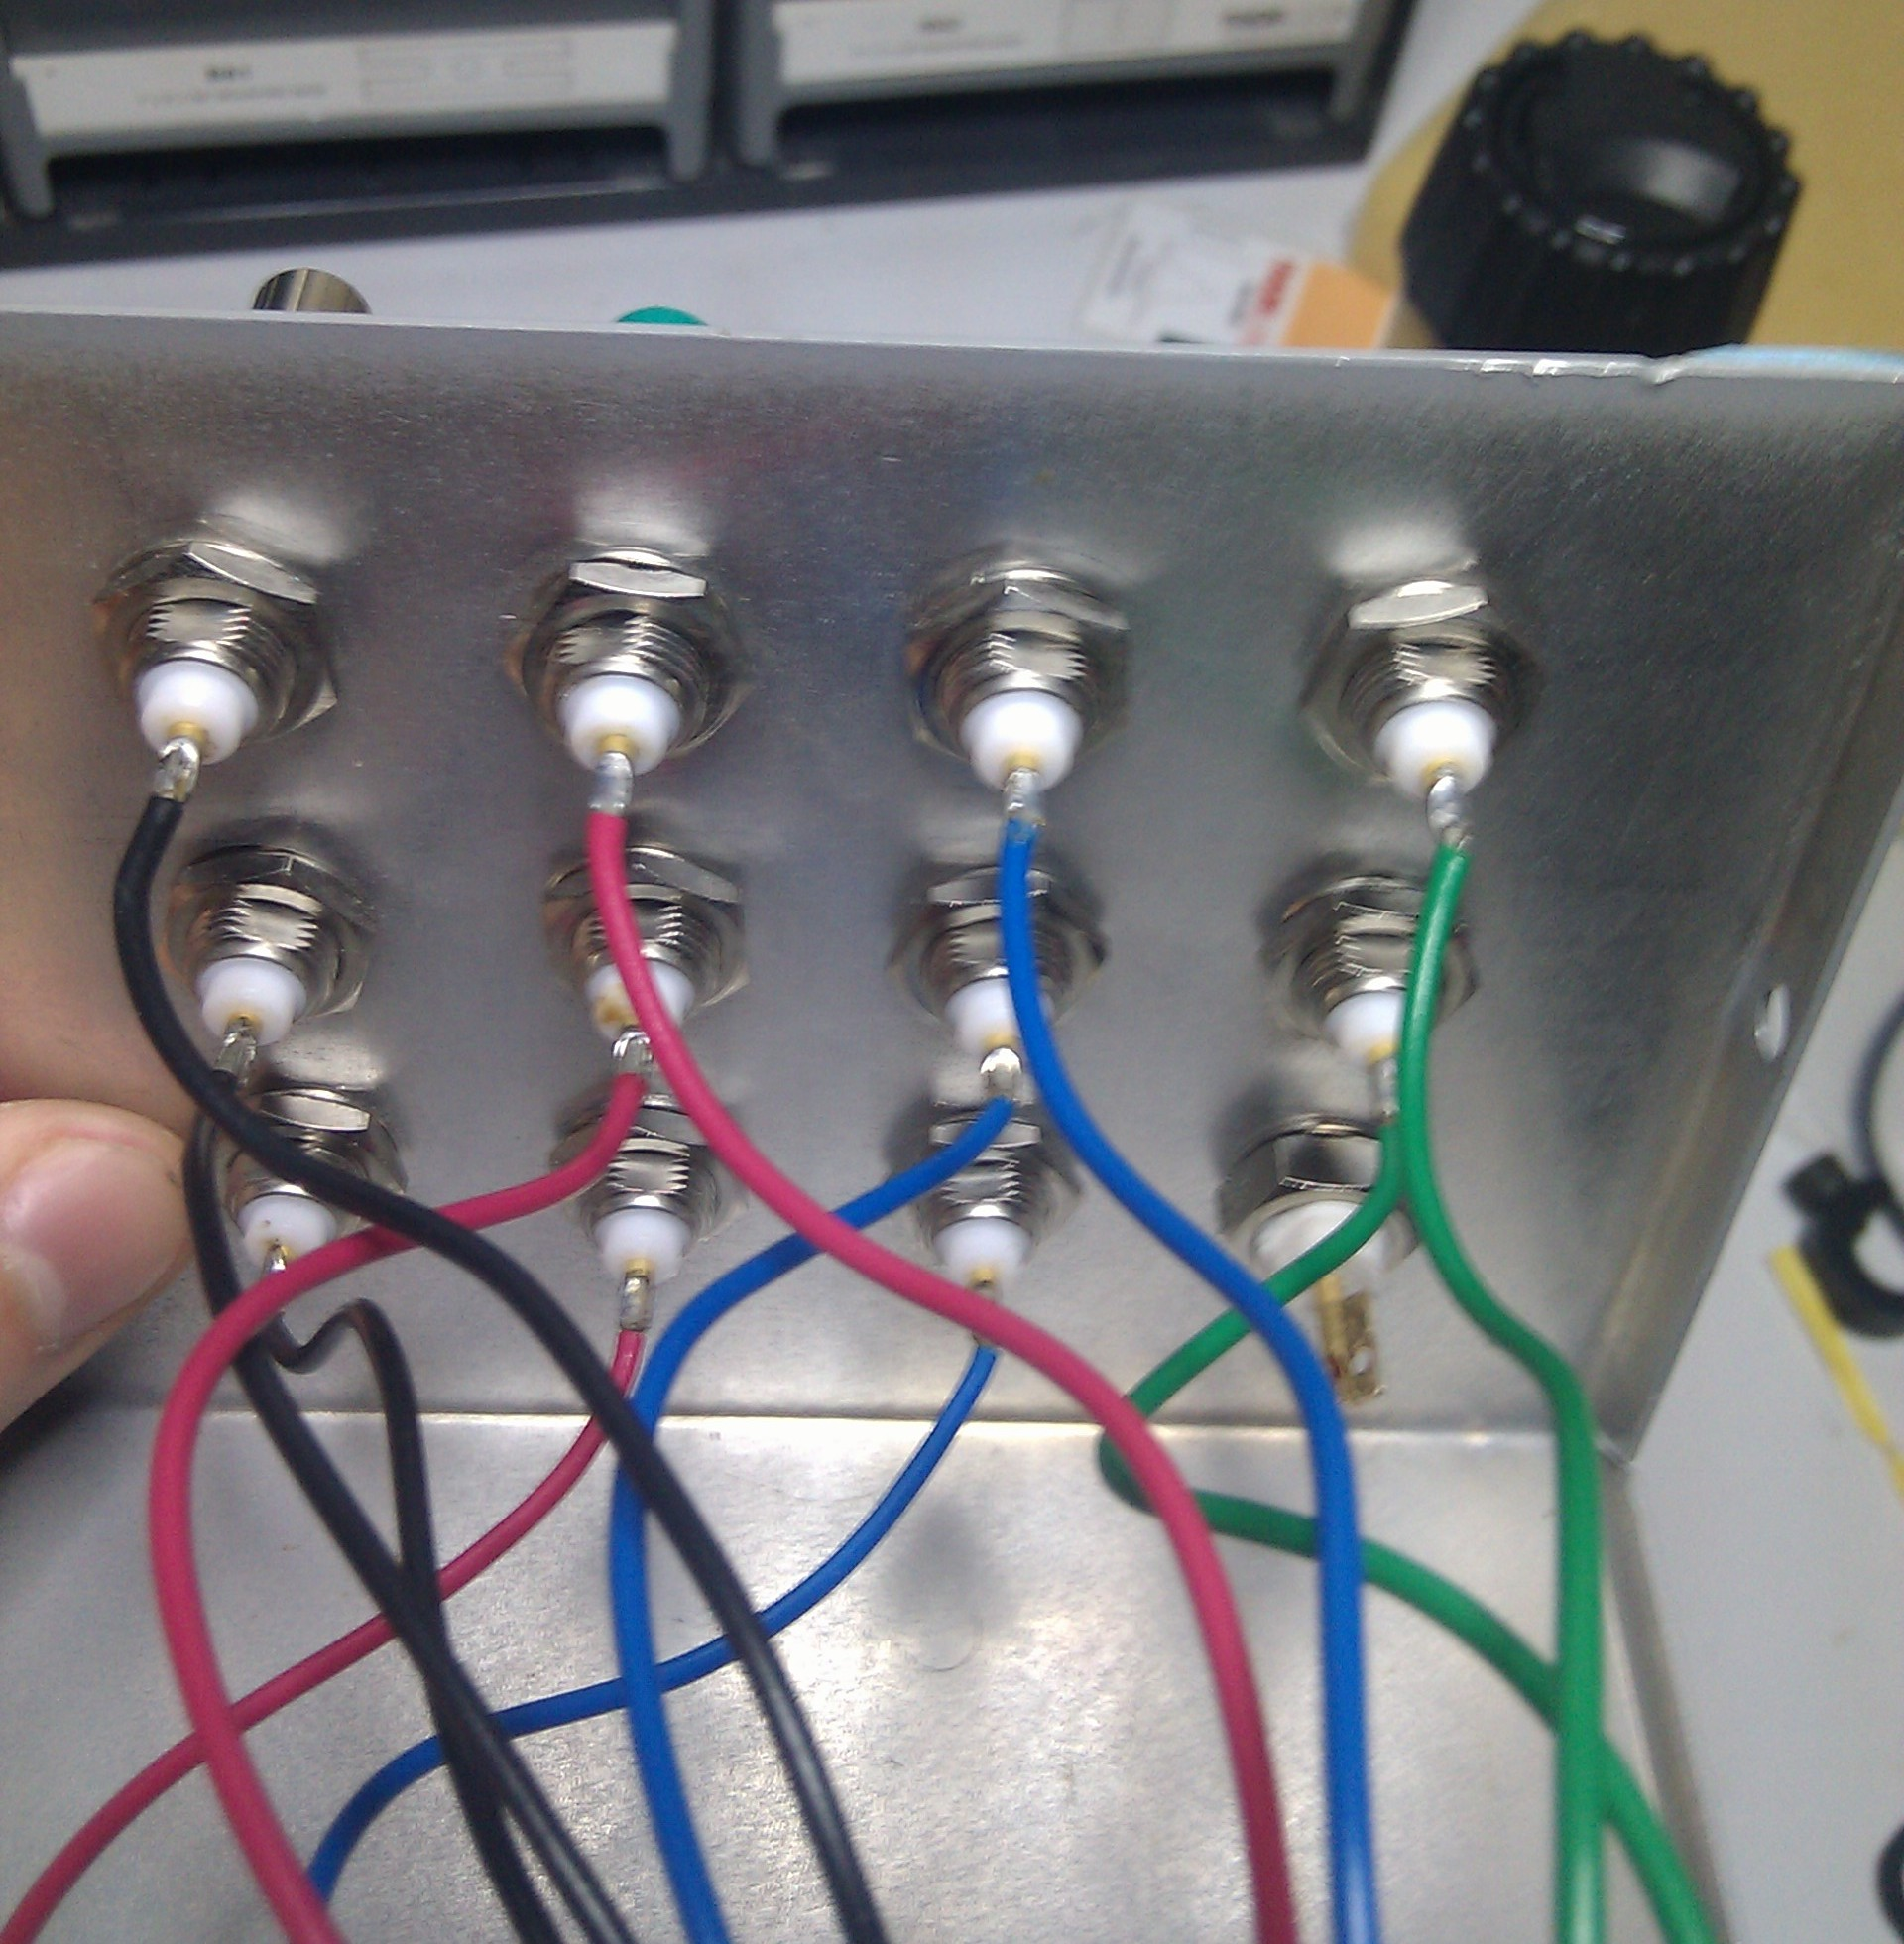
\includegraphics[scale=0.2]{connector-back.jpeg}
  \caption{Back side of the front panel}
  \label{fig:front-panel-rear}
\end{figure}

\begin{table}
  \center
  \begin{tabular}{|lcr|}
    \hline
    Name    & Direction & Pin Number \\
    \hline
    strobe0 & input  & 69 \\
    strobe1 & input  & 70 \\
    strobe2 & input  & 73 \\
    strobe3 & input  & 74 \\
    \hline
    delta0  & output & 79 \\
    delta1  & output & 92 \\
    delta2  & output & 93 \\
    delta3  & output & 97 \\
    \hline
  \end{tabular}
  \caption{Pin assignments in default firmware image.}
  \label{table:pins}
\end{table}


\section{External Crystal}

While it is technically possible to run the FPGA off of the clock
provided by the FX2, the characteristics of this clock are not
suitable for precise timing applications. For this reason, it is
highly recommended that an external crystal is installed. This is made
easy by the fact that the Xylo board provides room for a standard
half-size four-pin crystal oscillator. This location can be found
adjacent to the FPGA and is marked by white silkscreen outlining the
crystal package (see Figure \ref{fig:crystal}). It is recommended that
an 8MHz crystal is used.

\begin{figure}
  \center
  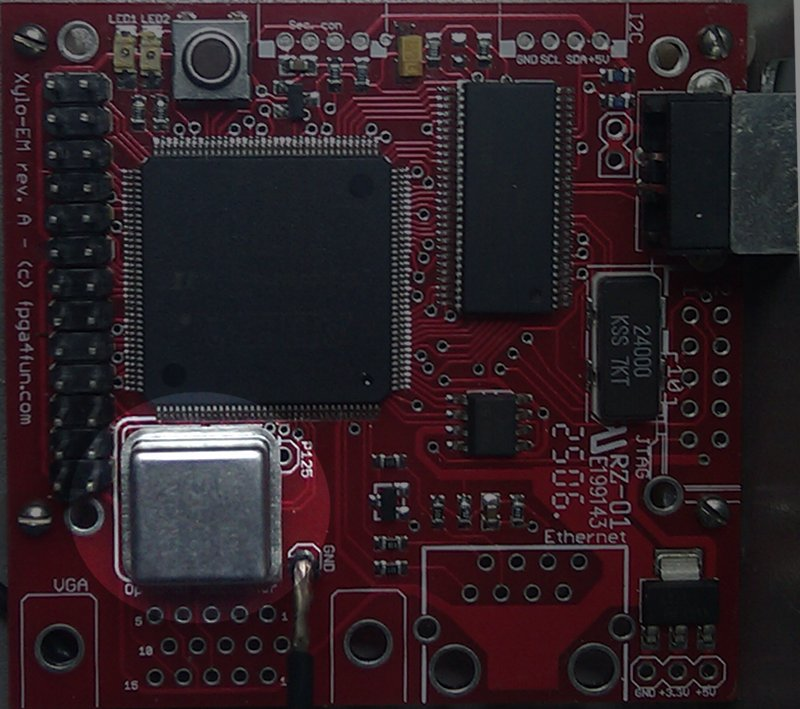
\includegraphics[scale=0.2]{oscillator.jpeg}
  \caption{Location of crystal oscillator pads}
  \label{fig:crystal}
\end{figure}

To mount a crystal, first determine pin 1 of the the crystal and its
associated hole on the board, marked by a sharp corner in the
silkscreen or metal package, respectively. Unfortunately, the board
has components directly beneath the crystal. Apply a piece of
insulating tape (e.g. Kapton) over these components to ensure they do
not short against the underside of the crystal. Place the crystal on
the board such that the four pins protrude the holes in the
board. Double check that the sharp corner of the package is aligned
with the sharp corner of the silkscreen. Finally, secure the crystal
in place with a piece of tape, turn the board over, and solder the
four pins.

\section{Uploading the bitstream}
\label{Sec:UploadingBitstream}

The logic on the FPGA is configured with a file called a bitstream.
If you are using the default clocking configuration (a 32.000 MHz
crystal multiplied up to 128MHz on the FPGA), you can use the 
precompiled bitstream found on the project website
\footnote{\url{http://goldnerlab.physics.umass.edu/~bgamari/timetag/timetag.rbf}}.
Otherwise see section \ref{Sec:ModifyingClock}.

\begin{figure}
  \center
  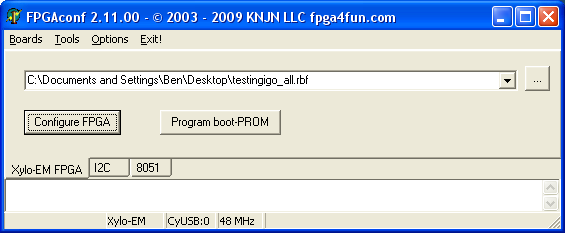
\includegraphics[scale=0.5]{fpgaconf.png}
  \caption{KNJN FPGA configuration utility}
  \label{fig:fpgaconf}
\end{figure}

Use the firmware upload tool ({\tt FPGAConf.exe}) provided by KNJN to
upload the bitstream to the Xylo's FLASH memory. You'll need a Windows
machine to run this tool.

\subsection{Modifying clock configuration}
\label{Sec:ModifyingClock}
If you wish to use a different clocking configuration, you'll need to
grab the firmware sources and compile your own bitstream. The clock
configuration is specified by the {\tt CLOCKRATE} variable in {\tt
config.v} and the multipliers {\tt clk0\_divide\_by} and {\tt
clk0\_multiply\_by} in {\tt altpll0.v}. In particular, these parameters
are related by,

\[ \mathtt{CLOCKRATE} = \frac{\mathtt{clk0\_multiply\_by}}{\mathtt{clk0\_divide\_by}} f_\mathrm{ext} \]

where $f_\mathrm{ext}$ is the frequency of the external crystal
oscillator. Of course, whenever the clocking configuration is changed,
it is necessary to ensure that the logic will still meet timing
constraints by running a timing simulation with Quartus.

\section{Done!}
You are done! Enjoy your timetagger.

\begin{comment}
\begin{figure}
  \center
  \includegraphics[scale=0.2]{T.jpeg}
  \caption{T the turtle says ``Hello!''.}
  \label{fig:T}
\end{figure}
\end{comment}

